\chapter{\label{ch:ch02}ПРАКТИЧЕСКАЯ ЧАСТЬ}

\section{\label{sec:ch01/sec01}Формулировка задачи}
Реализовать игровой процесс следующим образом. Предоставлено поле с редактируемыми размерами. Игроку предоставлено управление для перемещения танка по полю. По полю также перемещаются танки противника и пытаются уничтожить танк игрока. Осуществлено взаимное перемещение объектов относительно друг друга. В процессе игры игрок, уничтожая танки, получает очки, которые начисляются в общий счет. Задача игры - набрать наибольшее количество очков. Игра завершится, когда жизни игрока станут равны нулю.

Само игровое поле будет иметь возможность редактировать размер, состав и расположение объектов на ней, при это будет менять и размер окна программы.

\section{\label{sec:ch01/sec02}Математическая модель}

\subsection{\label{sec:ch01/sec03/sub01}Игровое меню}

Игровое меню - это то, с чего начинается программа сразу после запуска. Это будет окно размером 800*600 пикселей, содержащий на себе название игры и список кнопок, по которым будет происходить переход.

\subsection{\label{sec:ch01/sec03/sub03}Окно "Об игре"}

Это окно будет выводиться по нажатии кнопки "Об игре" в главном меню. Оно будет содержать информацию об управлении в игре и ФИО, группу студента, разработавшего данную программу.

\subsection{\label{sec:ch01/sec03/sub04}Игровое поле}

Это основной цикл в программе, в котором на холсте (окне игры) будут размещаться игровые объекты, происходить взаимодействия между объектами. Игроку будет предоставлено управление с клавиатуры.

Размер окна в этом разделе будет варьироваться от количества блоков игрового поля в ширину и высоту (количество блоков * размер блока) (но не равны нулю, само собой).

\section{\label{sec:ch02/sec03}Разработка}
\subsection{\label{sec:ch02/sec03/sub01}Математическая модель}

Программа будет состоять из нескольких файлов, каждый из которых представляет собой отдельный раздел (за исключением файла config.py)

Главное меню:

Создается основной файл main.py, с которого и будет осуществляться запуск програмы. Программа начинается с открытия главного меню. Создается окно, дается название (название игры), задается фиксированный размер 800x600 и центральное положение относительно экрана (далее о центральном положении не будет упоминаний, т.к. это выполняется для всех окон по умолчанию). Tkinter позволяет очень просто разместить виджеты в любой точке рабочего окна. Размещаются 4 кнопки друг под другом (с соответствующими заголовками). Они все будут выполнять функции, которые представляют собой открытия дочерних окон и работы в них.

Уже на этом этапе потребуется создать дополнительный файл config.py. Его задачей будет являться хранение констант для возможности быстрого доступа, например в программе часто будет фигурировать размер блока, возможность регулировать параметры игры: частота кадров, скорость игрока, врагов и снарядов.

Раздел "Об игре":

Как уже сказано ранее, этот раздел является функцией, которая открывает дочернее окно под названием about, которое, в свою очередь, находится в отдельном файле about.py. Всё, что оно должно делать, так это выводить текст с информацией о названии, управлении и авторе. Выход из раздела будет осуществлен нажатием на крестик в верхнем правом углу окна.

Раздел "Редактор карты":

Переход в этот раздел осуществляется через нажатие кнопки "Редактор карты". С помощью функции size открывается окно, с выбором размера для будущей карты в количестве блоков. После выбора или игнорирования (значения останутся по умолчанию 20, 20) можно нажать кнопку "Применить". В этом случае текущее окно закроется и откроется редактор. Редактор по внешнему виду напоминает игровой процесс, только область для вывода интерфейса с жизнями игрока и очками меняется на список блоков на выбор. Также добавляется кнопка "Сохранить изменения" и функция заполнения всего поля выбранным блоком. Среди блоков на выбор, помимо кирпичной и нерушимой стены можно увидеть танк игрока и пустой блок. Пустой блок позволяет очистить ячейку, а вместе с функцией заполнения позволяется очистить целое поле. Блок с танком игрока дает возможность разместить место появления игрока, но как можно догадаться, только одно, и для этого установлено ограничение, которое после нажатия кнопки "Сохранить изменения" проверит количество размещённых танков. В случае размещения более одного танка либо ни одного откроется окно с сообщением, уведомляющее о некоректном действии.

Игровой процесс:

Код самой игры расположен в файле game. Игровой процесс, по сути, является функцией под названием main. В начале этой функции идет процесс подготовки к игре, который включает в себя следующий алгоритм:
\begin{itemize}
\item Открытие файла map.txt (файл, содержащий данные о размере и расположении объектов на поле).
\item определение её размеров, открытие окна с вычисленными размерами.
\item Объявление 4-х классов:
    \begin{itemize}
    \item класс Bullet:

    Этот класс отвечает за отрисовку, движение и взаимодействие всех снарядов во время игры.
    
    Каждый объект при создании имеет инициализацию. Объект добавляется в список всех снарядов (bullets), ему даются начальные координаты x и y, направления движения vx и vy, определяется владелец снаряда ouner и рисуется сам снаряд на холсте game\_sc методом create\_oval.

    Метод update класса Bullet выполняет роль логики для движения и столновения снарядов. Каждый цикл метода update продвигает снаряд на определённые координаты (x/y=x/y+vx/vy) и методом move холста game\_sc перерисовывается в новых координатах. Далее идёт проверка на столкновения с краями поля и препятствиями.

    \item класс Enemy:
    Представляет собой логику всех вражеских танков в игре.
    
    При появлении танка выполняется метод инициализации. В нём создавшийся объект помещается в список enemies для упрощения контроля над ними. Метод принимает на вход координаты x, y, на которых должен появиться танк на поле, двумя координатами vx и vy задается скорость и направление танка. Аналогично со снарядами, танк рисуется на холсте game\_sc в заданных координатах x, y. Затем при помощи их методов задается начальное направление и зацикливаются действия стрельбы и случайного поворота.
    
    \textit{
    Очень важно упомянуть про зацикливание в Tkinter. У библиотеки есть функция after, которая выполняет любую другую функцию с любой задаваемой задержкой. В программе часто применяется следующий прием: внутрь функции, вызываемой функцией after, помещается такая же функция after. Получается, что при одиночном запуске функции, она начнёт выполняться бесконечно. Но эту бесконечность можно прерывать, просто поместив внутреннюю функцию в структуру if.}

    Метод rand\_change\_dir выполняет роль случайной смены направления. Метод основан на модели случайного блуждания клетки из книги Ю.Тарасевича "Математическое и компьютерное моделирование. Вводный курс"~\cite{book-math-mod}. Код реализации представлен на рисунке 2.1.

    \begin{figure}[h!]
        \centering
        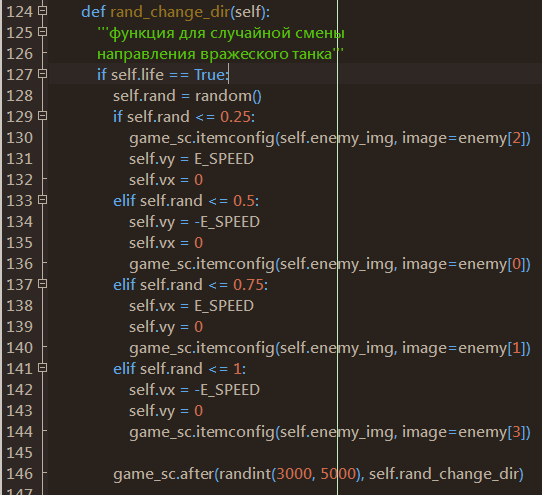
\includegraphics[width=0.8\textwidth]{./images/image3.png}
        \caption{\centering\label{fig:example05}Реализация метода rand\_change\_dir.}
    \end{figure}
    
    Метод shoot дает возможность врагам стрелять. Функция не принимает ничего, так как все требуемые переменные в области видимости метода. Реализация очень проста. В зависимости от текущего направления танка создается объект класса Bullet (т.е. снаряд) с координатами в центре изображения танка с тем же направлением.

    метод explosion играет только декоративную роль - эффект взрыва после уничтожения. Происходит это сменой изображения танка на три последовательных изображения взрыва с промежутком в значение переменной anim\_speed. Для отслеживания индекса изображения в инициализации танка добавлена переменная i.

    Последний и самый важный метод update отвечает за передвижение танков и проверку на столкновения. Алгоритм такой: сохранение текущих координат в переменных old\_x, old\_y, смещение координат на постоянную скорости vx и vy, новая позиция проверяется сначала на преодоление границ поля (x в пределах от 0 до WIDTH, y в пределах от 0 до HEIGHT), а затем на столкновение с объектами (прохождение по списку объектов и проверка пересечения квадратов этих объектов). В случае прохождения хотя бы по одному из этих циклов, выполняется уже описанная ранее функция случайного перемещения, которая принимает старые координаты объекта (во избежание застреваний). Последним шагом меняется положение изображения перемещаемого танка на новые координаты, либо старые, в случае столкновения.
    
    \end{itemize}
\item объявление 2-х функций.
    \begin{itemize}
    \item Функция случайной генерации врагов (enemy\_spawn). Она начинается с того, что создается список mass размером map\_width * map\_height и заполняется нулями. Затем при помощи логической переменной block\_free координаты всех объектов на поле проверяются на наличие этих объектов на каком-то блоке. Если таковые нашлись, то ячейка списка mass в остановленной координате сохраняет значение 0 и значение 1 в другом случае.

    Она определена независимо от класса Enemy, так как её вызов обратился бы к существующему обьекту класса, который должен быть создан, что вызовет противоречие и, вследствие, ошибку.
    \item Функция cooldown содержит единственную строку, которая обнуляет переменную shotTimer объекта player. Она вызывается при помощи метода after, чтобы осуществить функцию задержки выстрела. После выполнения этой функции задержка пропадает и позволяет игроку снова совершить выстрел.
    \end{itemize}
\item загрузка необходимых изображений. В них входят:
    \begin{itemize}
    \item Изображения блоков (brick - картинка кирпичной стены, armor - картинка непробиваемой стены).
    \item Изобржения игрока (tank - список из 4 картинок одного зелёного танка в 4 различных направлениях)
    \item Изображения врага (аналогично с изображениями игрока, но цвет танка красный)
    \item Изображения взрыва (bang - список из 3 изображений последовательно анимируемого взрыва)
    \item Изображение для визуального интерфейса (HUD), дающий игроку знать, какое количество жизней у него в запасе (lives).
    \end{itemize}
\item Расположение на окне 2-х холстов (один (interface) для отображения интерфейса, второй (game\_sc) для отображения игрового поля).
\begin{figure}[H]
    \centering
    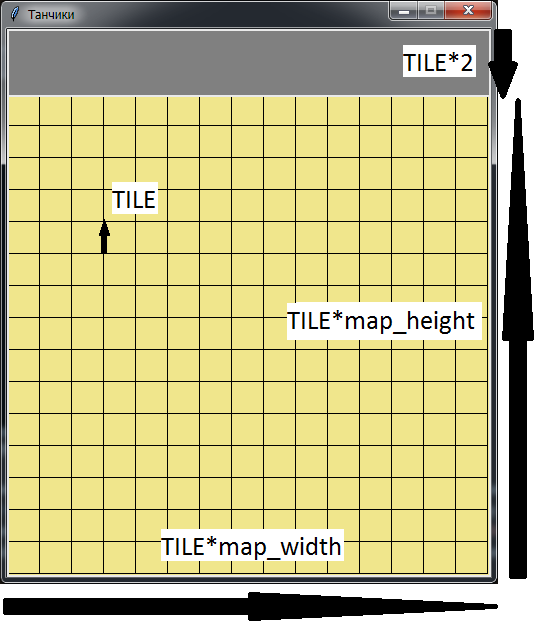
\includegraphics[width=0.5\textwidth]{./images/image1.png}
    \caption{\centering\label{fig:example05}Размещение холстов на игровом окне с размерами.}
\end{figure}

Холсты на окне размещаются в определённых размерах. Тот размер в блоках, что задаётся для игрового поля, является количество блоков, умноженные на длину одного блока (TILE). Панель интерфейса  расположена над игровым полем. Для неё выделено два блока в высоту Для размещения на нём количества жизней игрока и количество очков, начисляемые за уничтожение врагов. 
\item Заполнение холста game\_sc игровыми объектами. Имеется в виду расстановка кирпичных/непробиваемых блоков и места расположения игрока.

\begin{figure}[H]
    \centering
    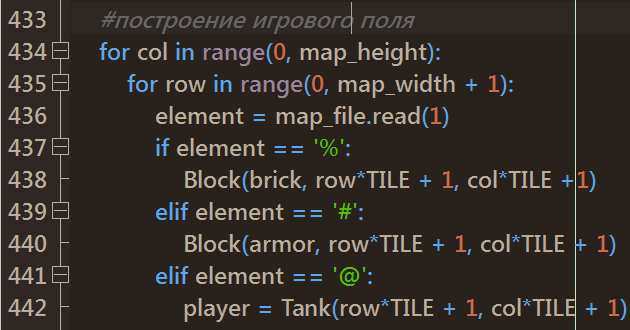
\includegraphics[width=0.5\textwidth]{./images/image2.png}
    \caption{\centering\label{fig:example05}Алгоритм размещения блоков и игрока на поле.}
\end{figure}

Это выполняется следующим образом: по вычисленным количествам блоков в ширину и длину выполняется двойной цикл for, который присваивает временной переменной прочтённый из файла map.txt символ, а затем, в зависимости от полученного символа выбирается установить вид блока на тех координатах, на которых в данный момент выполняется цикл.
\item Размещение на холсте interface надписи "Счет:", числа, обозначающего значение счета и кол-ва жизней игрока. Все они размещены с помощью виджета Label.
\item Циклом с пятью повторениями создание 5 врагов функцией enemy\_spawn.
\item Назначение функций движения игрока на клавиши. Функция move класса Tank назначается на нажатие любой клавиши клавиатуры "<Key>" (а уже внутри самой функции условия отсеивают нажатия конкретных клавиш), остановка движения функции stop определены на отпускание клавиш "<KeyRelease>", функция стрельбы игрока shoot назначена на нажатие кнопки пробела "<space>".
\item Объявление функции game. Это основной цикл игры, который за одну итерацию проходит по всем врагам, снарядам и игроку, чтобы выполнить однородный для всех объектов метод update. Чтобы возобновлять врагов после уничтожения и добавлять очки, применяется исловие на проверку длины списка врагов, в данном случае эта длина равна 4 и если окажется на один танк меньше (засчитано уничтожение), то будет переменная title\_score возрастет на 100 и появится новый враг посредством функции enemy\_spawn. Завершение игры должно произойти, когда кол-во жизней игрока станет равным 0, поэтому предлается следующая реализация функции game: метод after холста game\_sc, выполняя функцию game\_sc с очень маленьким промежутком (с задержкой в переменную FPS), создает эффект анимации. Чтобы избежать бесконечного зацикливания, внутри функции game добавляется условие равенства жизней игрока нулю, и в таком случае предлагается выйти из цикла или подготовить игру к завершению.
\end{itemize}

\subsection{\label{sec:ch01/sec03/sub04}
Блок-схема программы}

\begin{figure}[H]
    \centering
    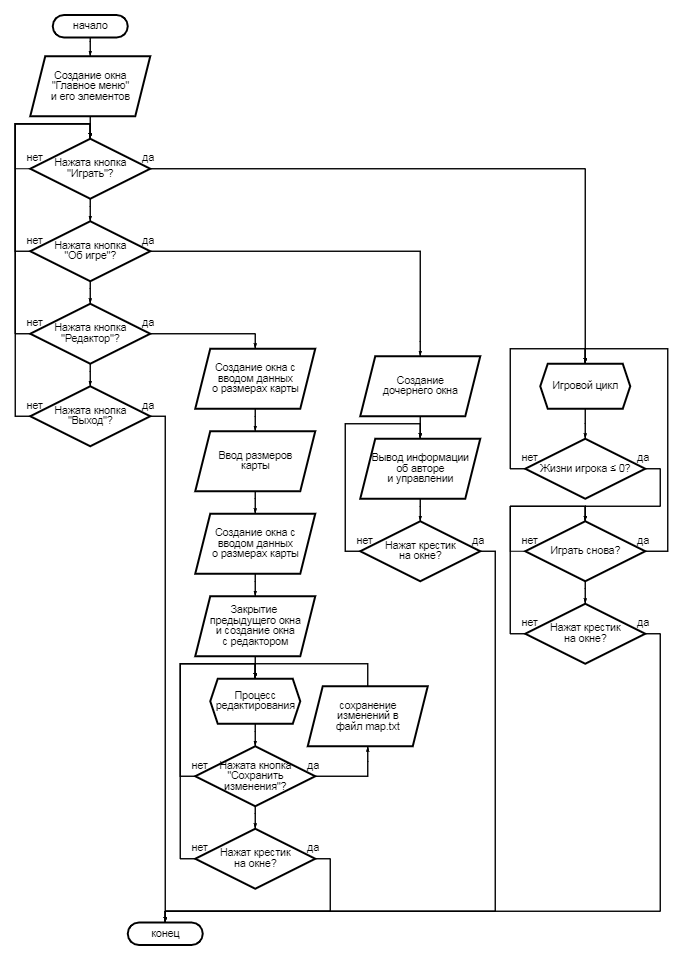
\includegraphics[width=1\textwidth]{./images/block-scheme.png}
    \caption{\centering\label{fig:example05}Блок-схема к программе "Танчики".}
\end{figure}

\subsection{\label{sec:ch01/sec03/sub04}
Написание кода программы}
Код программы приведён в пункте "Приложение".

\section{\label{sec:ch02/sec04}Тестирование}
Тестирование проводилось на операционных системах:
\begin{enumerate}
\item Windows
\item Linux
\end{enumerate}
На обеих ОС запуск программы прошёл успешно. Был проверен весь функционал программы: все кнопки выполняют конкретную функцию без ошибок, игра корректно запускается и завершается (выводится надпись "Игра окончена") Окна отображаются корректно.

\textit{Оказалось удобным, что при закрытии главного окна меню закрываются также все дочерние окна, т.е. все остальные.}

\begin{figure}[H]
    \centering
    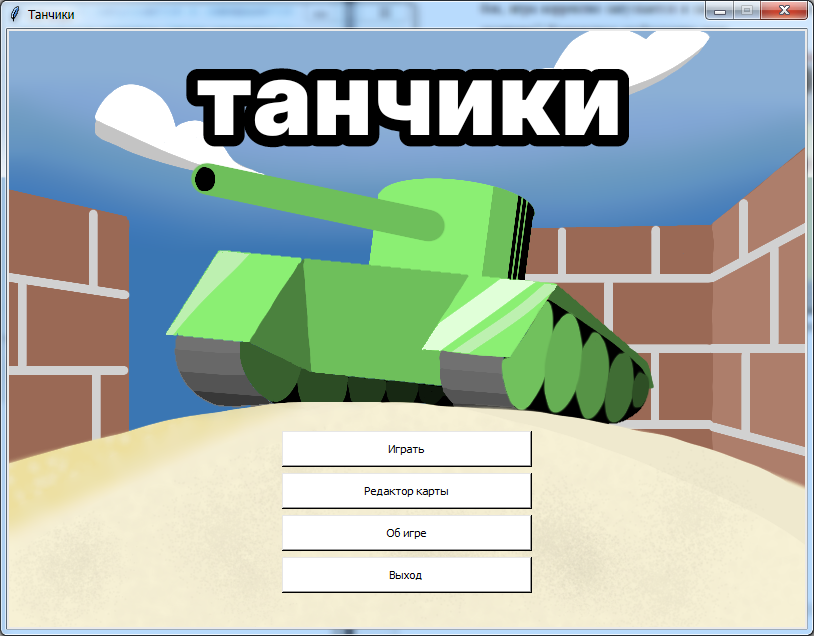
\includegraphics[width=0.7\textwidth]{./images/image5.png}
    \caption{\centering\label{fig:example05}Внешний вид главного меню.}
\end{figure}

\begin{figure}[H]
    \centering
    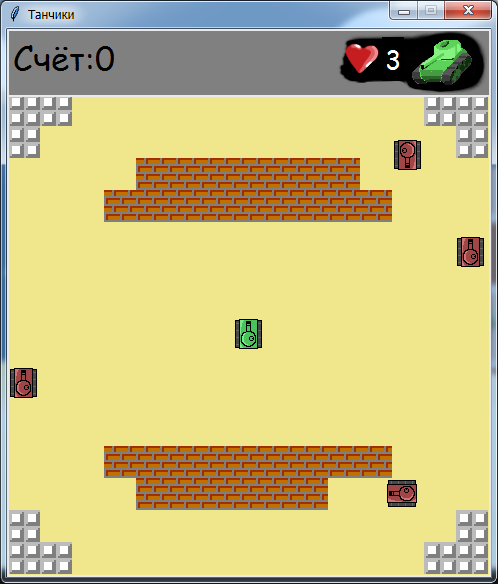
\includegraphics[width=0.5\textwidth]{./images/game_process.png}
    \caption{\centering\label{fig:example05}Внешний вид игрового процесса.}
\end{figure}

\begin{figure}[H]
    \centering
    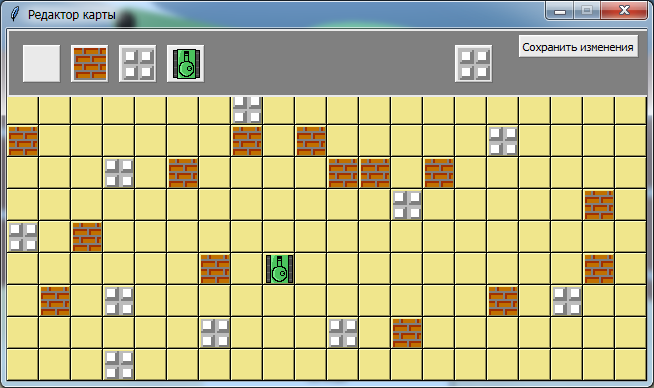
\includegraphics[width=0.7\textwidth]{./images/image4.png}
    \caption{\centering\label{fig:example05}Проверка работоспособности редактора.}
\end{figure}